\documentclass[aspectratio=169]{beamer}
\usetheme{simple}
\usepackage[english]{babel}
\usepackage[utf8]{inputenc} 
\usepackage{lmodern}
\usefonttheme[onlymath]{serif}
\usepackage[scale=2]{ccicons} 
\usepackage[makeroom]{cancel}
\usepackage{copyrightbox}

\usepackage{graphicx,hyperref,url,pgfplots}
\usepackage{amsmath} 
\usepackage{array,booktabs}
\pgfplotsset{compat=1.13}  
\usepackage{pifont}
\usepackage{bibentry}
\usepackage[alf,abnt-etal-list=0,abnt-etal-cite=3]{abntex2cite}
\usepackage[normalem]{ulem}

\usepackage[
    type={CC},
    modifier={by-nc-sa},
    version={4.0},
]{doclicense}

\setbeamercovered{invisible}
\newcommand{\pausar}{ }
\newcommand{\df}[1]{\,\mathrm{d}#1}
\newcommand{\parcial}[3]{\dfrac{\partial^{#1}#2}{\partial #3^{#1}}}
\newcommand{\cpright}[2]{\copyrightbox[b]{#1}{\tiny Source: #2}}
\newcommand{\cmark}{\textcolor{green}{\ding{51}}}%
\newcommand{\xmark}{\textcolor{red}{\ding{55}}}%

\usepackage{tikz}
\usepackage{xcolor}
\usetikzlibrary{scopes}
\usepackage{verbatim}
\usetikzlibrary{patterns}


\usepackage{listings}
  \lstdefinestyle{ascii-tree}{
    literate={├}{|}1 {─}{--}1 {└}{+}1 
  }
	\definecolor{codegreen}{rgb}{0,0.6,0}
	\definecolor{codegray}{rgb}{0.5,0.5,0.5}
	\definecolor{codepurple}{rgb}{0.58,0,0.82}
	\definecolor{backcolour}{rgb}{0.92,0.92,0.92}
	\lstset{language=Python, 
	backgroundcolor=\color{backcolour},   
	commentstyle=\color{codegreen},
	keywordstyle=\color{magenta},
	numberstyle=\tiny\color{codegray},
	stringstyle=\color{codepurple},
	basicstyle=\fontsize{8}{11}\ttfamily,
	frame=lines,
%	numbers=left, 
	tabsize=2,
	morekeywords={models, lambda, forms},
	showstringspaces=false}

\usepackage{catchfile}
\newcommand{\getenv}[2][]{%
    \CatchFileEdef{\temp}{"|kpsewhich --var-value #2"}{\endlinechar=-1}%
    \if\relax\detokenize{#1}\relax\temp\else\let#1\temp\fi}
\getenv[\RMHOME]{RM_HOME_PATH}

% --------------------------------------------------------------------------------------------

\title{Mobile Robots}
\subtitle{Robot Kinematics}
\date{\today}
\author[Jeferson José de Lima]{
  \textbf{Professor}: Jeferson José de Lima}
  \institute{Academic Department of Informatics (DAINF) \\ Federal University of Technology - Paraná (UTFPR) at Pato Branco, PR, Brazil}

\begin{document} 

\maketitle

\begin{frame}[t]{Useful Information}

    \begin{block}{License}
        \doclicenseThis
    \end{block}

	\begin{block}{links:}
		\begin{enumerate}
			\item \href{https://moodle.utfpr.edu.br/course/view.php?id=14218}{Moodle}
			\item \href{https://gitlab.com/cursoseaulas/robotica-movel/-/wikis/home}{Mobile Robots - Gitlab Page}
		\end{enumerate}
	\end{block}
    
\end{frame}


\begin{frame}{Modelos}
    \framesubtitle{Introdução}
    \begin{itemize}
        \item Tipo de Modelos:
              \begin{itemize} 
                  \item Modelo Cinemático;
                  \item Modelo Dinâmico;
              \end{itemize}
    \end{itemize}
    \begin{center}
        \begin{figure}
            \cpright{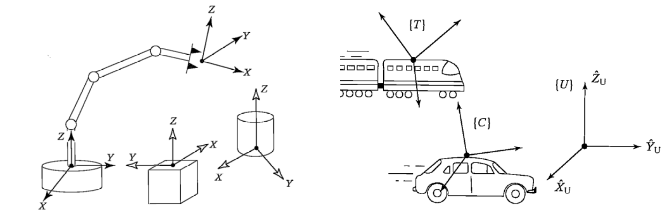
\includegraphics[width=0.9\textwidth]{./images/coord_frame.png}}
        {\cite{craig2009introduction}}
        \caption{Coordenadas do Sistema}
        \end{figure}
    \end{center}
\end{frame} 


\begin{frame}{Modelagem Cinemática}
    \framesubtitle{Conceitos}
    \begin{itemize}
        \item A cinemática é a área da Física que estuda o movimento dos corpos.
        \item Em robótica móvel a cinemática estabelece relações entre o deslocamento (locomoção) do robô e a atuação a ele imposta.
        \item A cinemática direta estabelece modelos que estimam o deslocamento do robô dada uma atuação, por exemplo, velocidade imposta às suas rodas. A cinemática direta está relacionada as \textbf{Coordenadas Generalizadas}.
        \item A cinemática inversa estabelece modelos que estimam a atuação necessária para que o robô realize um determinado deslocamento, por exemplo, percorrer uma trajetória \footnote{http://143.106.148.168:9080/Cursos/IA368N/01-16/cinematica2.pdf}.
    \end{itemize}
\end{frame}


\begin{frame}{Modelagem Cinemática}
    \framesubtitle{Introdução}
    Modelo Cinemático:
            \begin{itemize}
                \item Cinemático Direta e Inversa;
                \item Holonomicidade\footnote{O termo holonômico é atribuído a Hertz (Arnol'd and (Eds.), 1994) e significa "universal", "integral", "integrável" ( literalmente: holo = o todo, conjunto, totalidade - nomia = lei). Portanto, sistemas não-holonômicos podem ser interpretados como sistemas não integráveis. \textcolor{blue}{Definem-se como não-holonômicos sistemas com dimensão finita onde algum tipo de restrição é imposta a um ou mais estados do sistema.}}
            \end{itemize}

\end{frame}


\begin{frame}{Cinemática de Robôs}
    \framesubtitle{Conceitos}
    \textbf{Um robô é modelado como um corpo rígido}
        \begin{itemize}
            \item 3 variáveis $x, y,\phi$ (plano)
            \item 6 variáveis $x,y,z, \alpha, \beta, \phi$ (espaço)
        \end{itemize}
    Deve-se estabelecer uma relação entre o sistema de referencia local (robô) e o sistema de referencia global
        \begin{itemize}
            \item Sistema de Referencia global, exemplo $\{W\}$, ou $\{A\}$\footnote{O sistema de referência $\{A\}$(global) e $\{B\}$(local) serão usados como exemplos genéricos em aula};
            \item Referencial local, exemplo $\{M\}$, ou $\{B\}$;
        \end{itemize}
        \begin{center}
            \cpright{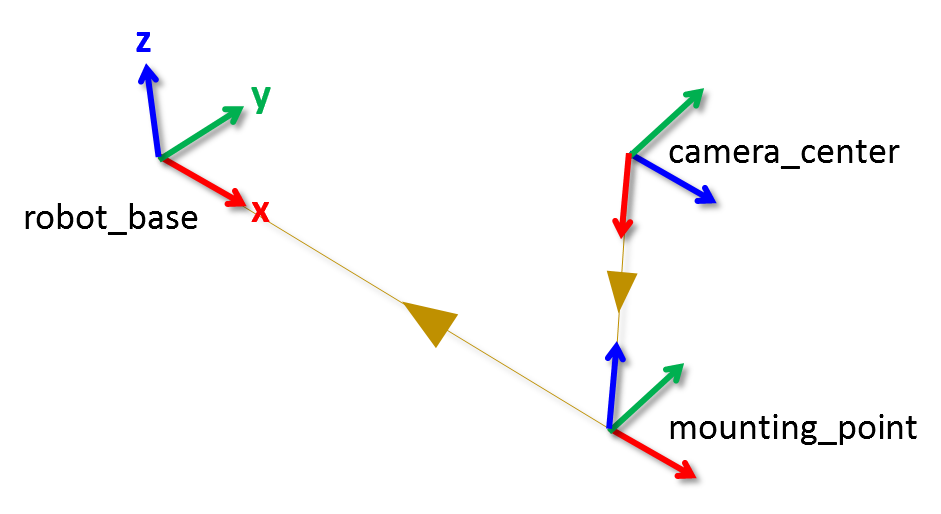
\includegraphics[width=0.4\textwidth]{./images/tf_1.png}}
            {https://www.kidscoding8.com/99205.html}
        \end{center}
\end{frame}



\begin{frame}{Modelagem Cinemática}
    \framesubtitle{Transformação homogênea - Conceitos}
    \begin{itemize}
        \item Um vetor de posição que pertence ao espaço $\mathbb{R}^{3 \times 1}$ é composto pelas coordenadas $X,Y$ e $Z$.
        \item Um ponto ${}^A\mathbf{P}$ representa a distância do vetor do plano $\{A\}$. Os elementos individuais de ${}^A\mathbf{P}$ podem ser visto pela equação \eqref{eq:cine1}.
    \end{itemize}
    \begin{columns}[c]
        \begin{column}{0.6\textwidth}
            \begin{figure}
                \centering
                \begin{tikzpicture}[scale=0.8]
                    \node(p0) at (0,0){};
                    \draw [->, blue] (p0.center) --++(0,3) node[right] {$ Y_A$};
                    \draw [->, rotate =120, blue] (p0.center) --++(0,3) node[below] {$ Z_A$};
                    \draw [->, rotate =240, blue] (p0.center) --++(0,3) node[below] {$ X_A$};
                    \draw [->, black] (p0.center) --++(2.5,0.5) node(B)[above,rotate=30] {${}^A\mathbf{P}$};
                    \node at (-1.5,2.5)[, blue] {$\{A\}$};
                \end{tikzpicture}
                \caption{Vetor em relação ao sistema de referências $\{A\}$}
                \label{fig:cine1f}
            \end{figure}
        \end{column}
        \begin{column}{0.3\textwidth}
            \begin{equation}\label{eq:cine1}
                \color{black}{{}^A\mathbf{P} = \begin{bmatrix}
                    p_x \\ p_y \\ p_z
                \end{bmatrix}}
                \color{gray}{}
            \end{equation}
        \end{column}
    \end{columns}
\end{frame}



\begin{frame}{Modelagem Cinemática}
    \framesubtitle{Transformação homogênea - Matriz de Rotação}
    \begin{itemize}
        \item O vetor definido por ${}^A\mathbf{P}$ pode ser rotacionado pela matriz de rotação $\mathbf{R}$, conforme a equação \eqref{eq:cine2}.
              \begin{equation}\label{eq:cine2}
                  {}_A^B
                  \mathbf{R} =
                  \begin{bmatrix}
                      r_{11} & r_{11} & r_{11} \\
                      r_{21} & r_{21} & r_{21} \\
                      r_{31} & r_{31} & r_{31} \\
                  \end{bmatrix}
              \end{equation}
    \end{itemize}

    \begin{block}{Considerando os exemplos}
        \begin{equation*}
            \mathbf{R}(\theta) =
            \begin{bmatrix}
                \cos \theta & -\sin \theta \\\sin \theta &\cos \theta
            \end{bmatrix}
        \end{equation*}
        ou:
        \begin{equation*}
            \mathbf{R}_z(\theta) =
            \begin{bmatrix}
                \cos(\theta) & -\sin(\theta) & 0 \\
                \sin(\theta) & \cos(\theta) & 0 \\
                0            & 0            & 1 \\
            \end{bmatrix} \text{, eixo $Z$ fixo}
        \end{equation*}
    \end{block}

\end{frame}


\begin{frame}[fragile]{Modelagem Cinemática}
    \framesubtitle{Transformação homogênea - Matriz de Rotação}
    \begin{itemize}
        \item Eigen is a C++ template library for linear algebra.
    \end{itemize}

    \begin{columns}
        \begin{column}[c]{0.4\textwidth}
        \begin{figure}
            \cpright{
\includegraphics[width=0.5\textwidth]{./images/eigen.jpeg}}
            {https://eigen.tuxfamily.org/}
        \end{figure}
        \end{column}
        \begin{column}[c]{0.6\textwidth}

	\begin{lstlisting}[language=C++]
#include <iostream>
#include <Eigen/Core>

int main(int argc, char* argv[])
{
  Eigen::Matrix<float, 2, 2> A;
  Eigen::Matrix<float, 2, 1> B;

  A << 0,    1,
       1,    1;
  B << 2,    2;

  std::cout << "A * B = \n" <<  A * B;
  return 0;
}

    \end{lstlisting}
        \end{column}
    \end{columns}


\end{frame}


\begin{frame}{Modelagem Cinemática}
    \framesubtitle{Transformação homogênea - Matriz de Rotação}
    \begin{itemize}
        \item Outros eixos:
    \end{itemize}
    \begin{block}{}
        \begin{equation*}
            \mathbf{R}_x(\theta) =
            \begin{bmatrix}
                1 & 0            & 0             \\
                0 & \cos(\theta) & -\sin(\theta) \\
                0 & \sin(\theta) & \cos(\theta)  \\
            \end{bmatrix} \text{, eixo $x$ fixo}
        \end{equation*}
        \begin{equation*}
            \mathbf{R}_y(\theta) =
            \begin{bmatrix}
                \cos(\theta)  & 0 & \sin(\theta) \\
                0             & 1 & 0            \\
                -\sin(\theta) & 0 & \cos(\theta) \\
            \end{bmatrix} \text{, eixo $y$ fixo}
        \end{equation*}
        \begin{equation*}
            \mathbf{R}_z(\theta) =
            \begin{bmatrix}
                \cos(\theta) & -\sin(\theta) & 0 \\
                \sin(\theta) & \cos(\theta) & 0 \\
                0            & 0            & 1 \\
            \end{bmatrix} \text{, eixo $z$ fixo}
        \end{equation*}
    \end{block}
\end{frame}


\begin{frame}[fragile]{Modelagem Cinemática}
    \framesubtitle{Transformação homogênea - Matriz de Rotação}
        \centering
        \begin{figure}
            \cpright{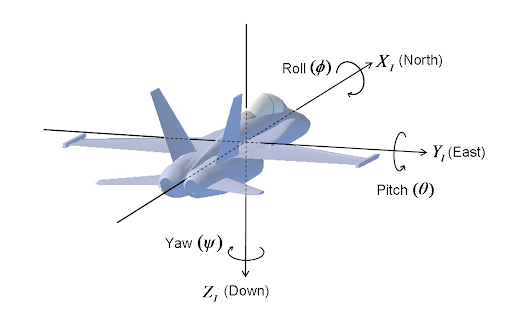
\includegraphics[width=0.5\textwidth]{./images/euler_angles.png}}
            {http://www.chrobotics.com/library/understanding-euler-angles}
        \end{figure}
        \begin{equation*}
            {\displaystyle \mathbf{R}_{z, y, x}=\mathbf{R}_{z}(\psi)\,\mathbf{R}_{y}(\phi )\,\mathbf{R}_{x}(\theta )={\overset {\text{yaw}}{\begin{bmatrix}\cos \psi &-\sin \psi &0\\\sin \psi &\cos \psi &0\\0&0&1\\\end{bmatrix}}}{\overset {\text{pitch}}{\begin{bmatrix}\cos \phi &0&\sin \phi \\0&1&0\\-\sin \phi &0&\cos \phi \\\end{bmatrix}}}{\overset {\text{roll}}{\begin{bmatrix}1&0&0\\0&\cos \theta &-\sin \theta \\0&\sin \theta &\cos \theta \\\end{bmatrix}}}}
        \end{equation*}
\end{frame}


\begin{frame}[fragile]{Modelagem Cinemática}
    \framesubtitle{Transformação homogênea - Matriz de Rotação}
        \centering
        \begin{figure}
            \cpright{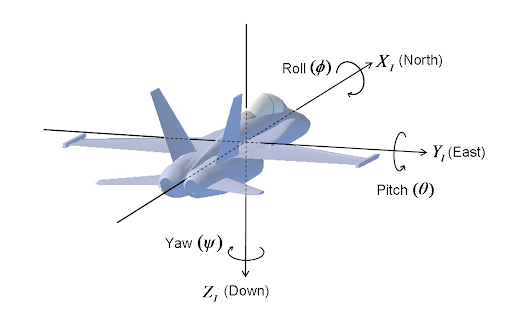
\includegraphics[width=0.5\textwidth]{./images/euler_angles.png}}
            {http://www.chrobotics.com/library/understanding-euler-angles}
        \end{figure}
    \begin{equation*}
        {\displaystyle  \mathbf{R}_{z, y, x}={\begin{bmatrix}\cos \psi \cos \phi &\cos \psi \sin \phi \sin \theta -\sin \psi \cos \theta &\cos \psi \sin \phi \cos \theta +\sin \psi \sin \theta \\\sin \psi \cos \phi &\sin \psi \sin \phi \sin \theta +\cos \psi \cos \theta &\sin \psi \sin \phi \cos \theta -\cos \psi \sin \theta \\-\sin \phi &\cos \phi \sin \theta &\cos \phi \cos \theta \\\end{bmatrix}}}
    \end{equation*}
\end{frame}

\begin{frame}[t]{Modelagem Cinemática}
    \framesubtitle{Transformação homogênea - Rotação de um coordenada}
    \begin{itemize}
        \item A rotação do sistema de referência $\{B\}$ em torno e $Z$, de um angulo qualquer $\theta$ em ${}^A\mathbf{P}$ é descrita como na equação \eqref{eq:cine3}, onde.
              \begin{equation}\label{eq:cine3}
                  {}^A\mathbf{P} = {}_B^A \mathbf{R}(\theta) {}^B\mathbf{P} =
                  \begin{bmatrix}
                      \cos(\theta) & -\sin(\theta) & 0 & 0 \\
                      \sin(\theta) & \cos(\theta) & 0 & 0 \\
                      0            & 0            & 1 & 0 \\
                      0            & 0            & 0 & 1 \\
                  \end{bmatrix}.
                  \begin{bmatrix}
                      {}^Ap_x \\
                      {}^Ap_y \\
                      {}^Ap_z \\
                      1
                  \end{bmatrix}
              \end{equation}
              \begin{columns}
                \begin{column}[c]{0.5\textwidth}
                \begin{figure}[!ht]
                    \centering
                    \begin{tikzpicture}[scale=0.5]
                        \node(p0) at (0,0){};
                        \draw [->] (p0.center) --++(0,3) node[right] {$\hat Y_A$};
                        \draw [->, rotate =120] (p0.center) --++(0,3) node[below] {$\hat Z_A$};
                        \draw [->, rotate =240] (p0.center) --++(0,3) node[below] {$\hat X_A$};
                        \node(p1) at (6,1){};
                        \draw [->, rotate =30, red] (p0.center) --++(0,3) node[right,rotate=30] {$\hat Y_B$};
                        \draw [->, rotate =150, red] (p0.center) --++(0,3) node[below,rotate=30] {$\hat Z_B$};
                        \draw [->, rotate =270, red] (p0.center) --++(0,3) node[below,rotate=30] {$\hat X_B$};
                        \draw [->, rotate =-20, red] (p0.center) --++(1.5,2) node(B)[above,rotate=30] {${}^B\mathbf{P}$};
                    \end{tikzpicture}
                \end{figure}
            \end{column}
            \begin{column}[c]{0.5\textwidth}
                A posição de ${}^A\mathbf{P}$ (sistema de referência global) em relação a ${}^B\mathbf{P}$ é encontrado através da multiplicação da matriz de ${}_B^A \mathbf{R}(\theta)$ (lê-se rotação do sistema de referência $B$ em $A$) pela posição de ${}^B\mathbf{P}$
            \end{column}
        \end{columns}
    \end{itemize}
\end{frame}

\begin{frame}[t]{Modelagem Cinemática}
    \framesubtitle{Transformação homogênea - Translação}
    \begin{itemize}
        \item Operador de translação $\mathbf{D}(q)$:
        \begin{columns}
            \begin{column}[c]{0.7\textwidth}
              \begin{figure}[!ht]
                  \centering
                  \begin{tikzpicture}[scale=0.6]
                      \node(p0) at (0,0){};
                      \draw [->] (p0.center) --++(0,3) node[right] {$\hat Y_A$};
                      \draw [->, rotate =120] (p0.center) --++(0,3) node[below] {$\hat Z_A$};
                      \draw [->, rotate =240] (p0.center) --++(0,3) node[below] {$\hat X_A$};
                      \node(p1) at (6,0.8){};
                      \draw [->, red] (p1.center) --++(0,3) node[right] {$\hat Y_B$};
                      \draw [->, rotate =120, red] (p1.center) --++(0,3) node[below] {$\hat Z_B$};
                      \draw [->, rotate =240, red] (p1.center) --++(0,3) node[below] {$\hat X_B$};
                      \draw [->, red] (p1.center) --++(2,2) node(B){};
                      \node[above] at (B.center) {${}^B\mathbf{P}_{p_x, p_y, p_z}$};
                      \draw [dotted,-latex] (p0)  -- (p1) node[midway, fill=white]{${}^A\mathbf{D}(q)$};
                      \draw [-latex,dashed] (p0)  -- (B.center) node[midway, fill=white]{${}^A\mathbf{P}$};
                      \node at (-1.5,2.5) {$\{A\}$};
                      \node at (4,2.5)[red] {$\{B\}$};
                  \end{tikzpicture}
              \end{figure}
            \end{column}
            \begin{column}[c]{0.3\textwidth}
                A operação de translação $\mathbf{D}(q)$ desloca a origem de ${}^B\mathbf{P}$ a partir do sistema referência $\{A\}$.
            \end{column}
        \end{columns}
    \end{itemize}

    \begin{equation}
        {}^A\mathbf{P} = {}^A\mathbf{D}(q) {}^B\mathbf{P} =
        \begin{bmatrix}
            1 & 0 & 0 & q_x \\
            0 & 1 & 0 & q_y \\
            0 & 0 & 1 & q_z \\
            0 & 0 & 0 & 1 \\
        \end{bmatrix}.
        \begin{bmatrix}
            p_x \\
            p_y \\
            p_z \\
            1
        \end{bmatrix}
    \end{equation}

\end{frame}


\begin{frame}{Modelagem Cinemática}
    \framesubtitle{Transformação homogênea - Translação}
    \begin{itemize}
        \item O Deslocamento é chamado de translação, e dá-se pelo operador translacional $\mathbf{D}_A(q)$, onde ${}^A\mathbf{Q}$ o incremento da posição em relação ao sistema de referencia $\{A\}$, conform equação \eqref{eq:cine4}.
              \begin{equation}\label{eq:cine4}
                  {}^A\mathbf{Q} =
                  \begin{bmatrix}
                      q_x \\ q_y \\ q_z
                  \end{bmatrix}, \qquad \mathrm{e} \qquad
                  \mathbf{D}_A =
                  \begin{bmatrix}
                      1 & 0 & 0 & q_x \\
                      0 & 1 & 0 & q_y \\
                      0 & 0 & 1 & q_z \\
                      0 & 0 & 0 & 1
                  \end{bmatrix}.
              \end{equation}
        \item Adota-se agora a notação para translação e rotação de um vetor, conforme a equação \eqref{eq:cine5}. Observa-se que o vetor ${}^A\mathbf{Q}$ foi incorporada pela nova notação.
              \begin{equation}\label{eq:cine5}
                  \begin{bmatrix}
                      {}^A\mathbf{P} \\ 1
                  \end{bmatrix}
                  =
                  \underbrace {
                      \left[
                          \begin{matrix}
                                & {}_B^A\mathbf{R} &   \\ \hline
                              0 & 0                & 0 \\
                          \end{matrix} \right.
                          \left.
                          \vline
                          \begin{matrix}
                              {}^A\mathbf{Q} \\ \hline
                              1
                          \end{matrix} \right]
                  }_{{}^A_B\mathcal{A}}
                  \begin{bmatrix}
                      {}^B\mathbf{P} \\
                      1
                  \end{bmatrix}
              \end{equation}
    \end{itemize}
\end{frame}


\begin{frame}{Modelagem Cinemática}
    \framesubtitle{Transformação homogênea - Operadores}
    \begin{itemize}
        \item Aplicando se uma transformação nas coordenada ${}^B\mathbf{P}$ pelos operadores de rotação e translação temos a representação de  ${}^A\mathbf{P}$
              \begin{figure}[!ht]
                  \centering
                  \begin{tikzpicture}[scale=0.7]
                      \node(p0) at (0,0){};
                      \draw [->] (p0.center) --++(0,3) node[right] {$\hat Y_A$};
                      \draw [->, rotate =120] (p0.center) --++(0,3) node[below] {$\hat Z_A$};
                      \draw [->, rotate =240] (p0.center) --++(0,3) node[below] {$\hat X_A$};
                      \node(p1) at (6,1){};
                      \draw [->, rotate =30, red] (p1.center) --++(0,3) node[right,rotate=30] {$\hat Y_B$};
                      \draw [->, rotate =150, red] (p1.center) --++(0,3) node[below,rotate=30] {$\hat Z_B$};
                      \draw [->, rotate =270, red] (p1.center) --++(0,3) node[below,rotate=30] {$\hat X_B$};
                      \draw [->, rotate =30, red] (p1.center) --++(1.5,4) node(B)[above,rotate=30] {${}^B\mathbf{P}$};
                      \draw [dotted,-latex] (p0)  -- (p1) node[midway, fill=white]{$\mathbf{P}_{BORG}$\footnote{A origem de sistema de referencia $\{B\}$ foi deslocada, conforme ${}^A\mathbf{Q}$}};
                      \draw [-latex,dashed] (p0)  -- (B) node[midway, fill=white]{${}^A\mathbf{P}$};;
                      \node at (-1.5,2.5) {$\{A\}$};
                      \node at (4,2.5)  [rotate=30, red]   {$\{B\}$};
                  \end{tikzpicture}
                  \label{fig:cine2}
              \end{figure}
    \end{itemize}
\end{frame}

\begin{frame}{Modelagem Cinemática}
    \framesubtitle{Transformação homogênea - Transformação Homogênea}
    \begin{itemize}
        \item Na forma generalizada, a transformação homogênea final ${}^{i}_0\mathbf{T}$ pode ser expressa pelo produto das sucessivas transformações de ${}^{i-1}_0\mathcal{A}_i$. Conforme é mostrado na equação \eqref{fig:cine3}.
              \begin{equation}\label{fig:cine3}
                  \begin{array}{lcl}
                      {}^i_0\mathbf{T} & = & {}^0_1\mathcal{A}{}^1_2\mathcal{A} \cdots {}^{i-1}_i\mathcal{A} = \prod \limits^i_{j=1}{}^{j-1}_i\mathcal{A}, \quad \mathrm{para\;}i=1,2,\cdots,n \\[.2cm]
                                       & = &
                      \begin{bmatrix}
                          x_i & y_i & z_i & p_i \\
                          0   & 0   & 0   & 1
                      \end{bmatrix} =
                      \begin{bmatrix}
                          {}^i_0\mathbf{R} & {}^i_0\mathbf{P} \\
                          \mathbf{0}       & 1
                      \end{bmatrix}
                  \end{array}
              \end{equation}
        \item onde, ${}^i_0\mathbf{P}$ é o vetor de orientação do referencial $i$ em relação a base $0$.
    \end{itemize}

\end{frame}

\begin{frame}{Modelagem Cinemática}
    \framesubtitle{Transformação homogênea - Exemplo}
    \begin{enumerate}
        \item Considerando que $\mathbf{v}_{t-1}$ é um vetor unitário em $\mathbf{v}_{t-1}=\{1,0,0\}$ e sofre um deslocamento de $\mathbf{Q}=\{2,1,0\}$ e rotação $\mathbf{R_z(\phi)}=20^o$, qual será a posição final de $v$ no plano $\{A\}$?
    \end{enumerate}
    \begin{columns}
        \begin{column}[c]{0.5\textwidth}
            \def\iangle{35} % Angle of the inclined plane
\def\down{0}
\def\arcr{0.7cm} % Radius of the arc used to indicate angles
\newcommand\centerofmass{%
    \tikz[radius=0.2em] {%
        \fill (0,0) -- ++(0.2em,0) arc [start angle=0,end angle=90] -- ++(0,-0.4em) arc [start angle=270, end angle=180];%
        \draw (0,0) circle;%
    }%
}

\begin{tikzpicture}[
    force/.style={>=latex,draw=blue,fill=blue},
    axis/.style={densely dashed,gray,font=\small},
    M/.style={rectangle,draw,fill=lightgray,minimum size=0.7cm,thin},
    m/.style={rectangle,draw=black,fill=lightgray,minimum size=0.3cm,thin},
    plane/.style={draw=black,fill=blue!10},
    string/.style={draw=red, thick},
    pulley/.style={thick},
    wheel/.style={fill=black, rounded corners=1.5pt},
]
     \begin{scope}[rotate=0]
        \node[M,transform shape] (M) at (-2,-1) {\centerofmass};
        % Draw axes and help lines
        {[axis,->]
            \draw (M) -- ++(0,2) node(y1_axis)[right] {$y'$};
        }
        % Forces
        {[force,->]
            % Assuming that Mg = 1. The normal force will therefore be cos(alpha)
            \draw (M.east) -- ++(1,0) node[above, blue] {$\mathbf{v}_{t-1}$};
        }
        \draw[wheel, fill=gray] (M.south west) rectangle ++(.4,-.1) node[]{};
        \draw[wheel, fill=gray] (M.north west) rectangle ++(.4,.1)  node[]{};
    \end{scope}


    %% Free body diagram of M
    \begin{scope}[rotate=\iangle]
        \node[M,transform shape] (M) {\centerofmass};
        % Draw axes and help lines
        {[axis,->]
            \draw (M) -- ++(0,2) node(y1_axis)[right] {$y'$};
            \draw (M) -- ++(2,0) node[right] {$x'$};
            % Indicate angle. The code is a bit awkward.
            \draw[solid,shorten >=0.5pt] (\down-\iangle:\arcr)
                arc(\down-\iangle:\down:\arcr);
            \node at (\down-0.5*\iangle:1.3*\arcr) {$\phi$};
        }
        % Forces
        {[force,->]
            % Assuming that Mg = 1. The normal force will therefore be cos(alpha)
            \draw (M.east) -- ++(1,0) node[above, blue] {$\mathbf{v}_t$};
        }
        \draw[wheel] (M.south west) rectangle ++(.4,-.1) node[below]{$v_D$};
        \draw[wheel] (M.north west) rectangle ++(.4,.1)  node[left]{$v_E$};
    \end{scope}
    % Draw gravity force. The code is put outside the rotated
    % scope for simplicity. No need to do any angle calculations. 
    \draw[axis,] (M.center) -- ++(1,0) node[below] {};
    %%
    \node[right, gray,font=\small, xshift=8] at (y1_axis) {$\{B\}$};
    %%
    \draw[, ->] (-2,-1) -- ++(4,0) node[below] {$x$};
    \draw[, ->] (-2,-1) -- ++(0,3) node(y_axis)[right] {$y$};
    \draw[gray, ->] (-2,-1) -- ++(-.5,-.5) node[left] {$z$};
    \node[left, gray,font=\small, xshift=-10] at (y_axis) {$\{A\}$};
\end{tikzpicture}

        \end{column}
        \begin{column}[c]{0.5\textwidth}
            \def\iangle{35} % Angle of the inclined plane
\def\down{0}
\def\arcr{0.7cm} % Radius of the arc used to indicate angles
\newcommand\centerofmass{%
    \tikz[radius=0.2em] {%
        \fill (0,0) -- ++(0.2em,0) arc [start angle=0,end angle=90] -- ++(0,-0.4em) arc [start angle=270, end angle=180];%
        \draw (0,0) circle;%
    }%
}

\begin{tikzpicture}[
    force/.style={>=latex,draw=blue,fill=blue},
    axis/.style={densely dashed,gray,font=\small},
    M/.style={rectangle,draw,fill=lightgray,minimum size=0.7cm,thin},
    m/.style={rectangle,draw=black,fill=lightgray,minimum size=0.3cm,thin},
    plane/.style={draw=black,fill=blue!10},
    string/.style={draw=red, thick},
    pulley/.style={thick},
    wheel/.style={fill=black, rounded corners=1.5pt},
]
    %% Free body diagram of M
    \begin{scope}[rotate=\iangle]
        \node[] (M) {};
%        \node[below, purple] at (M) {${}^B_A\mathbf{P}$};
        % Draw axes and help lines
        {[axis,->]
            \draw (M.center) -- ++(0,2) node(y1_axis)[right] {$y'$};
            \draw (M.center) -- ++(2,0) node[right] {$x'$};
            % Indicate angle. The code is a bit awkward.
            \draw[solid,shorten >=0.5pt] (\down-\iangle:\arcr)
                arc(\down-\iangle:\down:\arcr);
            \node[xshift=10, brown]at (\down-0.5*\iangle:1.3*\arcr) {$\mathbf{R}_z(\phi)$};
        }
        % Forces
        {[force,->]
            % Assuming that Mg = 1. The normal force will therefore be cos(alpha)
            \draw (M.center) -- ++(1,0) node[above, blue] {$\mathbf{v}_{t}$};
        }
    \end{scope}
    % Draw gravity force. The code is put outside the rotated
    % scope for simplicity. No need to do any angle calculations. 
    \draw[axis,] (M.center) -- ++(1,0) node[below] {};
    %%
    \node[right, gray,font=\small, xshift=8] at (y1_axis) {$\{B\}$};
    %%
    \draw[, ->] (-2,-1) -- ++(4,0) node[below] {$x$};
    \draw[, ->] (-2,-1) -- ++(0,3) node(y_axis)[right] {$y$};
    \draw[gray, ->] (-2,-1) -- ++(-.5,-.5) node[left] {$z$};
    \node[left, gray,font=\small, xshift=-10] at (y_axis) {$\{A\}$};
    \draw [densely dashed,red,] (-2,-1)-- (M.center) node[above, midway] {${}^A\mathbf{Q}$};
    \draw [force,->](-2,-1) -- ++(1,0) node[below, blue] {$\mathbf{v}_{t-1}$};
\end{tikzpicture}

  
        \end{column}
    \end{columns}
    Transformação Homogênea:
    \begin{equation*}
        \begin{bmatrix}
            \color{purple}{{}^A \mathbf{v}_{t}} \\ 1
        \end{bmatrix}
        =
        \left[
            \begin{matrix}
                  & \color{brown}{{}_B^A\mathbf{R}_z(\phi)} &   \\ \hline
                0 & 0                                       & 0 \\
            \end{matrix} \right.
            \left.
            \vline
            \begin{matrix}
                \color{red}{{}^A\mathbf{Q}} \\ \hline
                1
            \end{matrix} \right]
        \begin{bmatrix}
            {}^B \mathbf{v}_{t-1} \\
            1
        \end{bmatrix}
    \end{equation*}
\end{frame}

\begin{frame}[t]{Modelagem Cinemática}
    \framesubtitle{Transformação homogênea - Resumo}
    \begin{itemize}
        \item \textcolor{purple}{\textbf{Resumo:}}
    \end{itemize}
    \begin{figure}
        \centering
        \cpright{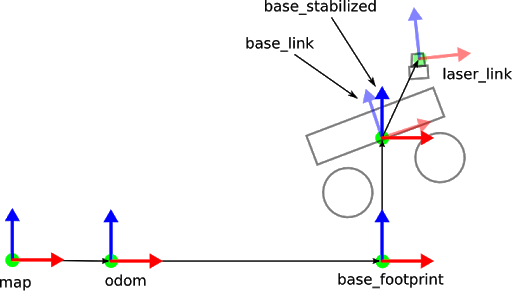
\includegraphics[width=0.5\textwidth]{./images/tf_2.png}}
        {https://answers.ros.org/questions/265846/revisions/}
        \caption{Exemplo de sistemas de referência - Carro}
    \end{figure}
\end{frame}

\begin{frame}[t]{Modelagem Cinemática}
    \framesubtitle{Transformação homogênea - Resumo}
    \begin{itemize}
        \item \textcolor{purple}{\textbf{Resumo:}}
    \end{itemize}
    \begin{figure}
        \centering
        \cpright{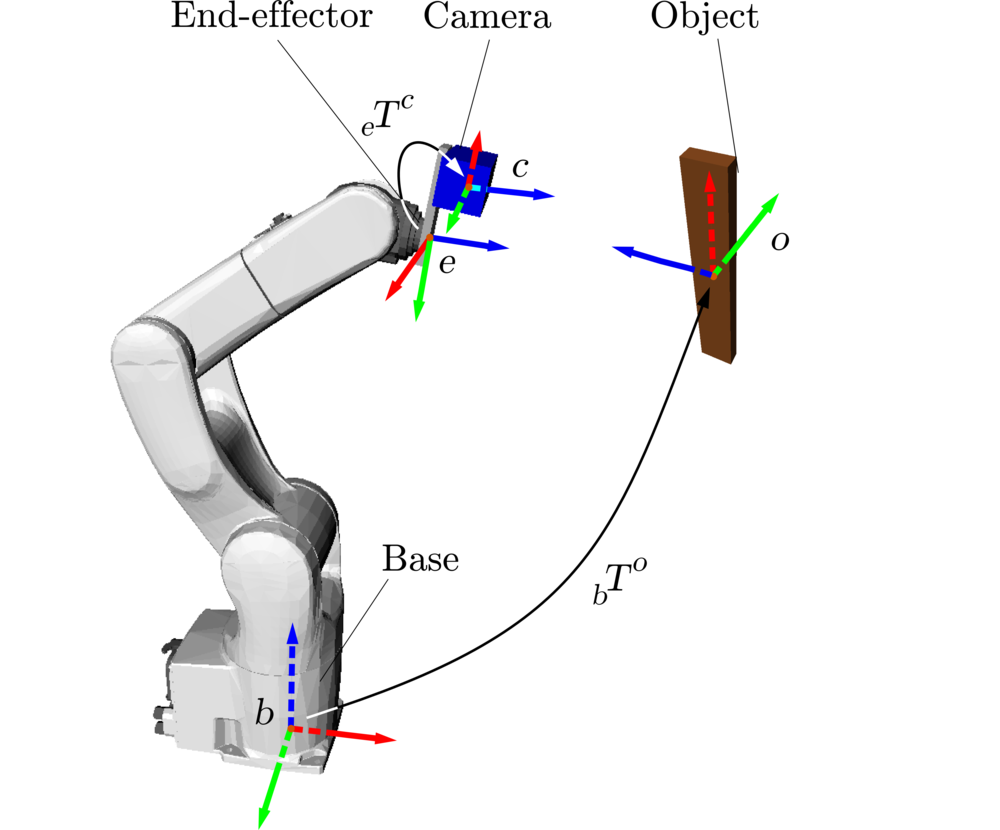
\includegraphics[width=0.4\textwidth]{./images/tf_3.png}}
        {http://www.osrobotics.org/osr/planning/introduction.html}
        \caption{Exemplo de sistemas de referência - Manipulador Robótico}
    \end{figure}
\end{frame}

\begin{frame}{Cinemática Direta e Inversa}
    \framesubtitle{Coordenadas Generalizadas}
    \begin{itemize}
        \item Considerando um robô fixo ou móvel com coodenadas generalizadas $q_1, q_2,..., q_n$ localizadas no espaço das \textcolor{red}{juntas ou atuadores (\textit{joint space}) $\mathbf{q}$}. Bem como $x_1, x_2,..., x_n$, o \textcolor{blue}{espaço das tarefas (\textit{task space}) $\mathbf{x}$}, temos então os vetores:
             \begin{equation*}
                \color{red}{
                  \mathbf{q} =
                  \begin{bmatrix}
                      q_1 \\q_2 \\ \cdots  \\ q_n
                  \end{bmatrix}
                }
                  \text{, }
                \color{blue}{
                  \mathbf{x} =
                  \begin{bmatrix}
                      x_1 \\x_2 \\ \cdots \\ x_n
                  \end{bmatrix}
                }
              \end{equation*}

        \item \textbf{Cinemática Direta e Inversa}. A \textcolor{red}{Cinemática Direta} descreve o estado do robô em função de entradas como (velocidade das rodas, movimento das juntas, direção das rodas ...).  A partir da \textcolor{blue}{Cinemática Inversa}, é possível projetar um planejamento de movimento, o que significa que as entradas do robô podem ser calculadas para uma sequência de estado do robô desejada.

    \end{itemize}
\end{frame}

\begin{frame}{Cinemática Direta e Inversa}
    \framesubtitle{Coordenadas Generalizadas}
    \begin{itemize}
        \item A relação entre as Cinemática Direta e Cinemática Inversa é obtida através da Matriz Jacobiana do Robô.

              \begin{equation*}
                  \mathbf{\dot{x}} = \mathbb{J}{\mathbf{\dot{q}}}
                  \text{ e, }
                  \mathbf{\dot{q}} = \mathbb{J}^{-1}{\mathbf{\dot{x}}}
              \end{equation*}

              bem como:

              \begin{equation*}
                  \frac{\text{d}\mathbf{x}}{\text{d}t} = \mathbb{J}\frac{\text{d}\mathbf{q}}{\text{d}t}
                  \text{ e, }
                  \frac{\text{d}\mathbf{q}}{\text{d}t} = \mathbb{J}^{-1}\frac{\text{d}\mathbf{x}}{\text{d}t}
              \end{equation*}

              onde $\mathbb{J}$ é dado por:
              \begin{equation*}
                  \mathbb{J}
                  =
                  \frac{d \mathbf{f}}{d \mathbf{q}}
                  =
                  \left[ \frac{\partial \mathbf{f}}{\partial q_1}
                      \cdots \frac{\partial \mathbf{f}}{\partial q_n} \right]
                  =
                  \begin{bmatrix}
                      \frac{\partial f_1}{\partial q_1} & \cdots &
                      \frac{\partial f_1}{\partial q_n}                   \\
                      \vdots                            & \ddots & \vdots \\
                      \frac{\partial f_m}{\partial q_1} & \cdots &
                      \frac{\partial f_m}{\partial q_n}
                  \end{bmatrix}
              \end{equation*}
    \end{itemize}
\end{frame}

\begin{frame}{Robot kinematics}
    \framesubtitle{Conceitos}
    \begin{itemize}
        \item O modelo cinemático não leva em conta a inércia do robô, deformações em
              sua estrutura, forças oriundas do deslocamento (atrito, escorregamento, etc.),
              e demais fatores internos e externos que possam afetar a locomoção.
        \item Os modelos dinâmicos são capazes de incorporar estas variáveis, mas são
              muito mais complexos que os modelos cinemáticos.
        \item Os modelos cinemáticos são suficientes quando a locamoção se dá a baixas
              velocidades e em piso plano e horizontal que propicie contato adequado para
              não haver escorregamento.
        \item Apesar do modelo cinemático ser inerentemente um modelo aproximado,
              podemos corrigir seus resultados a partir dos sensores do robô. Os algoritmos
              de localização robótica fazem exatamente isto.\href{http://143.106.148.168:9080/Cursos/IA368N/01-16/cinematica2.pdf}{[1]}
    \end{itemize}
\end{frame}

\begin{frame}{Robot kinematics}
    \framesubtitle{Diversos modelos de cinemática}
    \begin{itemize}
        \item \textbf{Cinemática Externa} descreve a posição do robô e orientação com relação ao sistema de referência externo, como por exemplo a relacao entre o robô e as coordenadas de um mapa global.
        \item \textbf{Cinemática Interna} Há a possibilidade também, da referência ser o próprio robô ou em relação as rodas.
        \item \textbf{Restrições de movimento} aparecem quando um sistema tem menos váriáveis de entrada do que graus de liberdade (DOF's).
    \end{itemize}
\end{frame}


\begin{frame}{Robot kinematics}
    \framesubtitle{Cinemática Externa}
    \begin{itemize}
        \item O deslocamento de um robô deve ser expresso em relação a um sistema de
              coordenadas (referencial) inercial (global). No plano, utilizamos coordenadas
              cartesianas (eixos X e Y).
    \end{itemize}

    \begin{columns}
        \begin{column}[c]{0.5\textwidth}
            \def\iangle{35} % Angle of the inclined plane
\def\down{0}
\def\arcr{0.7cm} % Radius of the arc used to indicate angles
\newcommand\centerofmass{%
    \tikz[radius=0.2em] {%
        \fill (0,0) -- ++(0.2em,0) arc [start angle=0,end angle=90] -- ++(0,-0.4em) arc [start angle=270, end angle=180];%
        \draw (0,0) circle;%
    }%
}

\begin{tikzpicture}[
    force/.style={>=latex,draw=blue,fill=blue},
    axis/.style={densely dashed,gray,font=\small},
    M/.style={rectangle,draw,fill=lightgray,minimum size=0.7cm,thin},
    m/.style={rectangle,draw=black,fill=lightgray,minimum size=0.3cm,thin},
    plane/.style={draw=black,fill=blue!10},
    string/.style={draw=red, thick},
    pulley/.style={thick},
    wheel/.style={fill=black, rounded corners=1.5pt},
]
    %% Free body diagram of M
    \begin{scope}[rotate=\iangle]
        \node[M,transform shape] (M) {\centerofmass};
        % Draw axes and help lines
        {[axis,->]
            \draw (M) -- ++(0,2) node(y1_axis)[right] {$y_M$};
            \draw (M) -- ++(2,0) node[right] {$x_M$};
            % Indicate angle. The code is a bit awkward.
            \draw[solid,shorten >=0.5pt] (\down-\iangle:\arcr)
                arc(\down-\iangle:\down:\arcr);
            \node at (\down-0.5*\iangle:1.3*\arcr) {$\phi_M$};
        }
        % Forces
        {[force,->]
            % Assuming that Mg = 1. The normal force will therefore be cos(alpha)
            \draw (M.east) -- ++(1,0) node[above, blue] {$v_M$};
        }
        \draw[wheel] (M.south west) rectangle ++(.4,-.1) node[below]{$v_{M_R}$};
        \draw[wheel] (M.north west) rectangle ++(.4,.1)  node[left]{$v_{M_L}$};
    \end{scope}
    % Draw gravity force. The code is put outside the rotated
    % scope for simplicity. No need to do any angle calculations. 
    \draw[axis,] (M.center) -- ++(1,0) node[below] {};
    %%
    \node[right, gray,font=\small, xshift=8] at (y1_axis) {$\{M\}$};
    %%
    \draw[, ->] (-2,-1) -- ++(4,0) node[below] {$x_I$};
    \draw[, ->] (-2,-1) -- ++(0,3) node(y_axis)[right] {$y_I$};
    \draw[gray, ->] (-2,-1) -- ++(-.5,-.5) node[left] {$z_I$};
    \node[left, gray,font=\small, xshift=-10] at (y_axis) {$\{I\}$};
\end{tikzpicture}

        \end{column}
        \begin{column}[c]{0.5\textwidth}
            \def\iangle{35} % Angle of the inclined plane
\def\down{0}
\def\arcr{0.7cm} % Radius of the arc used to indicate angles
\newcommand\centerofmass{%
    \tikz[radius=0.2em] {%
        \fill (0,0) -- ++(0.2em,0) arc [start angle=0,end angle=90] -- ++(0,-0.4em) arc [start angle=270, end angle=180];%
        \draw (0,0) circle;%
    }%
}

\begin{tikzpicture}[
    force/.style={>=latex,draw=blue,fill=blue},
    axis/.style={densely dashed,gray,font=\small},
    M/.style={rectangle,draw,fill=lightgray,minimum size=0.7cm,thin},
    m/.style={rectangle,draw=black,fill=lightgray,minimum size=0.3cm,thin},
    plane/.style={draw=black,fill=blue!10},
    string/.style={draw=red, thick},
    pulley/.style={thick},
    wheel/.style={fill=black, rounded corners=1.5pt},
]
    %% Free body diagram of M
    \begin{scope}[rotate=\iangle]
        \node[] (M) {};
%        \node[below, purple] at (M) {${}^B_A\mathbf{P}$};
        % Draw axes and help lines
        {[axis,->]
            \draw (M.center) -- ++(0,2) node(y1_axis)[right] {$y_M$};
            \draw (M.center) -- ++(2,0) node[right] {$x_M$};
            % Indicate angle. The code is a bit awkward.
            \draw[solid,shorten >=0.5pt] (\down-\iangle:\arcr)
                arc(\down-\iangle:\down:\arcr);
            \node[xshift=10, brown]at (\down-0.5*\iangle:1.3*\arcr) {$\mathbf{R}_z(\phi)$};
        }
        % Forces
        {[force,->]
            % Assuming that Mg = 1. The normal force will therefore be cos(alpha)
            \draw (M.center) -- ++(1,0) node[above, blue] {$v_M$};
        }
    \end{scope}
    % Draw gravity force. The code is put outside the rotated
    % scope for simplicity. No need to do any angle calculations. 
    \draw[axis,] (M.center) -- ++(1,0) node[below] {};
    %%
    \node[right, gray,font=\small, xshift=8] at (y1_axis) {$\{M\}$};
    %%
    \draw[, ->] (-2,-1) -- ++(4,0) node[below] {$x_I$};
    \draw[, ->] (-2,-1) -- ++(0,3) node(y_axis)[right] {$y_I$};
    \draw[gray, ->] (-2,-1) -- ++(-.5,-.5) node[left] {$z_I$};
    \node[left, gray,font=\small, xshift=-10] at (y_axis) {$\{I\}$};
    \draw [densely dashed,red,] (-2,-1)-- (M.center) node[above, midway] {${}^A\mathbf{Q}$};
\end{tikzpicture}

  
        \end{column}
    \end{columns}

    \begin{equation*}
        \begin{bmatrix}
            \color{purple}{x_I} \\ \color{purple}{y_I} \\ \color{purple}{z_I}\\1
        \end{bmatrix}
        =
        \begin{bmatrix}
            \color{purple}{{}^M_I\mathbf{P}} \\ 1
        \end{bmatrix}
        =
        \left[
            \begin{matrix}
                  & \color{brown}{{}_M^I\mathbf{R}_z(\phi)} &   \\ \hline
                0 & 0                                       & 0 \\
            \end{matrix} \right.
            \left.
            \vline
            \begin{matrix}
                \color{red}{{}^I\mathbf{Q}} \\ \hline
                1
            \end{matrix} \right]
        \begin{bmatrix}
            {}^M\mathbf{P} \\
            1
        \end{bmatrix}
    \end{equation*}

\end{frame}


\begin{frame}{Robot kinematics}
    \framesubtitle{Cinemática Interna}
    \begin{columns}
        \begin{column}[c]{0.5\textwidth}
            \begin{figure}
                \def\iangle{35} % Angle of the inclined plane
\def\down{0}
\def\arcr{0.7cm} % Radius of the arc used to indicate angles
\newcommand\centerofmass{%
    \tikz[radius=0.2em] {%
        \fill (0,0) -- ++(0.2em,0) arc [start angle=0,end angle=90] -- ++(0,-0.4em) arc [start angle=270, end angle=180];%
        \draw (0,0) circle;%
    }%
}

\begin{tikzpicture}[
    force/.style={>=latex,draw=blue,fill=blue},
    axis/.style={densely dashed,gray,font=\small},
    M/.style={rectangle,draw,fill=lightgray,minimum size=0.7cm,thin},
    m/.style={rectangle,draw=black,fill=lightgray,minimum size=0.3cm,thin},
    plane/.style={draw=black,fill=blue!10},
    string/.style={draw=red, thick},
    pulley/.style={thick},
    wheel/.style={fill=black, rounded corners=1.5pt},
]
    %% Free body diagram of M
    \begin{scope}[rotate=\iangle]
        \node[M,transform shape] (M) {\centerofmass};
        % Draw axes and help lines
        {[axis,->]
            \draw (M) -- ++(0,1.3) node(y1_axis)[right] {$y$};
            \draw (M) -- ++(2,0) node[right] {$x$};
            % Indicate angle. The code is a bit awkward.
            \draw[solid,shorten >=0.5pt] (\down-\iangle:\arcr)
                arc(\down-\iangle:\down:\arcr);
            \node at (\down-0.5*\iangle:1.3*\arcr) {$\phi$};
        }
        % Forces
        {[force,->]
            % Assuming that Mg = 1. The normal force will therefore be cos(alpha)
            \draw (M.east) -- ++(1,0) node[above, blue] {$v_R$};
        }
        \draw[wheel] (M.south west) rectangle ++(.4,-.1) node[below]{$v_{D}$};
        \draw[wheel] (M.north west) rectangle ++(.4,.1)  node[left]{$v_{E}$};
        \draw [dotted, -](M) -- ++(0,2) node(CIR)[above] {CIR};
        \node[below,  yshift=-10, xshift=-5] at (CIR) {$\omega$};
    \end{scope}
    % Draw gravity force. The code is put outside the rotated
    % scope for simplicity. No need to do any angle calculations. 
    \draw[axis,] (M.center) -- ++(1,0) node[below] {};
    %%
    \node[right, gray,font=\small, xshift=8] at (y1_axis) {$\{R\}$};
    %%
    \draw[, ->] (-2,-1) -- ++(4,0) node[below] {$X$};
    \draw[, ->] (-2,-1) -- ++(0,3) node(y_axis)[right] {$Y$};
    \draw[gray, ->] (-2,-1) -- ++(-.5,-.5) node[left] {$Z$};
    \node[left, gray,font=\small, xshift=-10] at (y_axis) {$\{M\}$};
\end{tikzpicture}
                \caption{Mobile Robot and the Instantaneous Center of Rotation (ICR)}
            \end{figure}
        \end{column}
        \begin{column}[c]{0.5\textwidth}
            \centering
            \begin{itemize}
                \item Position:
                      \newline

                      $\mathbf{x} = \begin{bmatrix}
                              x \\
                              y
                          \end{bmatrix}$
                      \newline

                \item Configuration Space (Localization and Orientation):
                      \newline

                      $\mathbf{q} =
                          \begin{bmatrix}
                              x \\
                              y \\
                              \phi
                          \end{bmatrix}$
            \end{itemize}
        \end{column}
    \end{columns}
\end{frame}


\begin{frame}{Robot kinematics}
    \framesubtitle{Robô Diferencial}
    \begin{itemize}
        \item Analisando a velocidade angular de $\omega$, temos:

              \begin{equation*}
                  \begin{split}
                      \omega & = \frac{v_L(t)}{R(t)-\frac{L}{2}} \\
                      \omega & = \frac{v_R(t)}{R(t)+\frac{L}{2}} \\
                  \end{split}
              \end{equation*}

              logo:

              \begin{equation*}
                  \begin{split}
                      \omega (t) = \frac{ v_R(t) - v_L(t)}{L} & \text{, e }
                      R(t)  = \frac{L v_R(t) + v_L(t)}{2 v_R(t) - v_L(t)} \\
                  \end{split}
              \end{equation*}

              assim, a velocidade tangencial do veiculo é dada por:

              \begin{equation}
                  v (t) =\omega (t) R(t) = \frac{ v_R(t) + v_L(t)}{2}
              \end{equation}
    \end{itemize}
\end{frame}



\begin{frame}{Robot kinematics}
    \framesubtitle{Robô Diferencial}
    \begin{itemize}
        \item As velocidades tangenciais $v_L(t)=r\omega_L(t)$ e $v_R(t)=r\omega_R(t)$, temos então a cinemática interna do robô (\textcolor{red}{coordenadas locais}):

              \begin{equation*}
                  \boxed{
                      \begin{bmatrix}
                          \dot{x}_M(t) \\
                          \dot{y}_M(t) \\
                          \dot{\phi}(t)
                      \end{bmatrix}
                      =
                      \begin{bmatrix}
                          \dot{v}_M(t) \\
                          \dot{v}_M(t) \\
                          \dot{\omega}(t)
                      \end{bmatrix}
                      =
                      \begin{bmatrix}
                          \frac{r}{2}  & \frac{r}{2} \\
                          0            & 0           \\
                          -\frac{r}{L} & \frac{r}{L}
                      \end{bmatrix}
                      \begin{bmatrix}
                          \omega_L(t) \\
                          \omega_R(t)
                      \end{bmatrix}}
              \end{equation*}

        \item e em \textcolor{red}{coordenadas globais}:

              \begin{equation*}
                  \boxed{
                      \begin{bmatrix}
                          \dot{x}(t) \\
                          \dot{y}(t) \\
                          \dot{\phi}(t)
                      \end{bmatrix}
                      =
                      \begin{bmatrix}
                          \cos(\phi(t)) & 0 \\
                          \sin(\phi(t)) & 0 \\
                          0             & 1
                      \end{bmatrix}
                      \begin{bmatrix}
                          v(t) \\
                          \omega(t)
                      \end{bmatrix}}
              \end{equation*}

              onde as variáveis $v(t)$ e $\omega(t)$


    \end{itemize}
\end{frame}


\begin{frame}{Robot kinematics}
    \framesubtitle{ From Continuous-Time Domain to Microcontroller Code}
    \begin{itemize}
        \item  We can be written in discrete form using Euler integration and evaluated at discrete time
        instants $t = kTs$ , $k = 0, 1, 2, \cdots$ where $T$ s is the following sampling interval:

              \begin{equation*}
                  \begin{split}
                      x_{k+1} &= x_k + v_k T_s\cos(\phi_k) \\
                      y_{k+1} &= y_k + v_k T_s\sin(\phi_k) \\
                      \phi_{k+1} &= \phi_k + \omega_k T_s \\
                  \end{split}
              \end{equation*}
    \end{itemize}
\end{frame}


\begin{frame}{Robot Kinematics}
    \framesubtitle{Motion Control - Open Loop Control}
    \begin{columns}
        \begin{column}[c]{0.5\textwidth}
            \begin{figure}
                \cpright{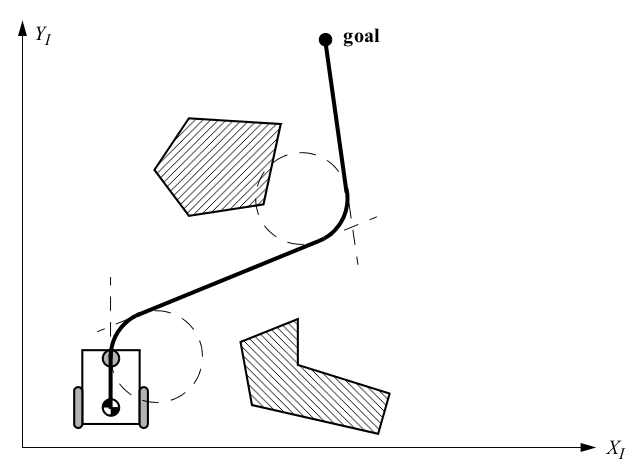
\includegraphics[width=0.9\textwidth]{./images/openloopcontrol.png}}
                {\cite{siegwart2011introduction}}
                \caption{Open-loop control of a mobile robot based on straight lines and circular trajectory segments}
            \end{figure}
        \end{column}
        \begin{column}[c]{0.5\textwidth}
            \centering
            \begin{itemize}
                \item Open Loop Control is often done by dividing the trajectory (path) in
                motion segments of clearly defined shape, for example, straight lines and segments of a circle.
            \end{itemize}
        \end{column}
    \end{columns}
\end{frame}

\begin{frame}{Robot Kinematics}
    \framesubtitle{Kinematic Control - Feedback Control}
    \begin{columns}
        \begin{column}[c]{0.5\textwidth}
            \begin{figure}
                \cpright{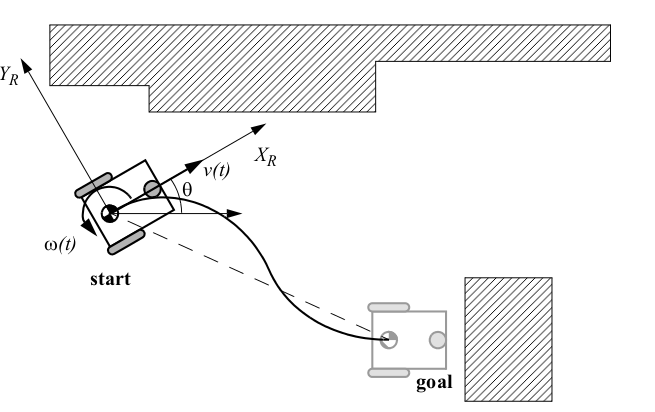
\includegraphics[width=0.9\textwidth]{./images/feedbackcontrol.png}}
                {\cite{siegwart2011introduction}}
                \caption{Typical situation for feedback control of a mobile robot}
            \end{figure}
        \end{column}
        \begin{column}[c]{0.5\textwidth}
            \centering
            \begin{itemize}
                \item The robot will not automatically adapt or correct the trajectory if dynamic changes of the environment occur.
                \item The resulting trajectories are usually not smooth, because the transitions from one trajectory segment to another are, for most of the commonly used segments (e.g., lines and part of circles), not smooth. 
                \item \textcolor{purple}{This means there is a discontinuity in the robot’s acceleration.}
            \end{itemize}
        \end{column}
    \end{columns}
\end{frame}


\begin{frame}{Robot Kinematics}
    \framesubtitle{Kinematic Control - Feedback Control}
    \begin{columns}
        \begin{column}[c]{0.4\textwidth}
            \begin{figure}
                \cpright{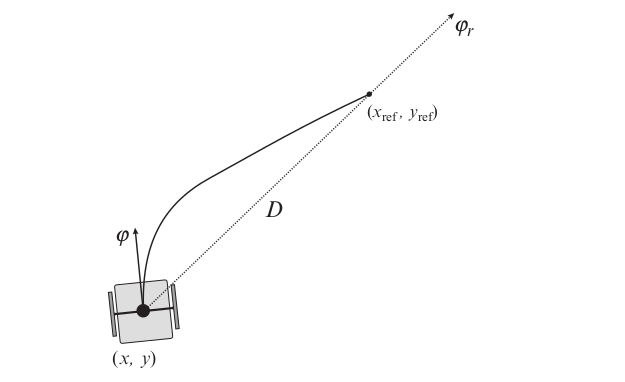
\includegraphics[width=1\textwidth]{./images/feedbackcontrol_2.png}}
                {\cite{siegwart2011introduction}}
                \caption{Feedback Control to reference position}
            \end{figure}
        \end{column}
        \begin{column}[c]{0.6\textwidth}
            \textbf{The robot feedback control}:
            \begin{itemize}
                \item \textcolor{blue}{Angular Velocity errors}:
                \begin{equation*}
                    \varphi_r(t) = \arctan\left( \frac{y_{ref}(t) - y(t)}{x_{ref}(t) - x(t)}\right)
                \end{equation*}

                \begin{equation*}
                    \omega(t) = K_{p_1} \left( \varphi_r(t) - \varphi(t) \right)
                \end{equation*}

                \item \textcolor{blue}{Linear Velocity errors}:
                
                \begin{equation*}
                    v(t) = K_{p_2} \sqrt{\left( x_{ref}(t) - x(t)\right)^2   + \left( y_{ref}(t) - y(t)\right)^2  }
                \end{equation*}
                
                \textcolor{purple}{where $K_{p_1}$ and $K_{p_2}$ is the Proportional Gain}
            \end{itemize}
        \end{column}
    \end{columns}
\end{frame}

\begin{frame}[fragile]{Robot kinematics}
    \framesubtitle{Kinematic Control - Code Examples: Feedback Control}

    \textbf{Project Example}:
    \begin{itemize}
        \item \href{https://gitlab.com/jeferson.lima/diff_drive_controller}{\textcolor{blue}{\textbf{Differential Drive Controller}}}
    \end{itemize}   
\end{frame}


\begin{frame}{Robot kinematics}
    \framesubtitle{Robôs Omnidirecional}
    continuar ...
\end{frame}

\begin{frame}{Robot kinematics}
    \framesubtitle{Robôs Com Esteiras}
    continuar ...
\end{frame}

  
\begin{frame}[t, allowframebreaks]
	\frametitle{Bibliography}
	\bibliography{\RMHOME/references.bib}
\end{frame}
  


\end{document} 
